\documentclass[11pt,a4paper]{article}
\usepackage[T1]{fontenc}
\usepackage[utf8]{inputenc}
\usepackage[spanish,es-noshorthands]{babel}
\usepackage[margin=2.5cm]{geometry}
\usepackage{enumitem}
\usepackage{url}
\usepackage{graphicx}
\graphicspath{{figs/}}
\setlist{itemsep=2pt}

\title{Menú 1: pedestal y ruido del Citiroc}
\author{JJ}
\date{\today}

\begin{document}
\maketitle

\section*{Aperitivo}

\begin{enumerate}
\item Tarjeta CAEN A5202 (dos Citiroc~1A, 64 canales),
leída a través del concentrador DT5215 con el programa de adquisición de
datos (DAQ) de JMB.
\item Uso los nombres que JMB define en su DAQ, que en todo caso, coinciden con los del software de CAEN (Janus, Sección~\ref{sec:janus}). 
\item El DAQ trabaja en modo peak stretch (programa de festejos, nota 0).
\end{enumerate}

\section{Medida del pedestal y el ruido}
\label{sec:medida}

\subsection*{La cadena del Citiroc}

\begin{figure}[!h]
\centering
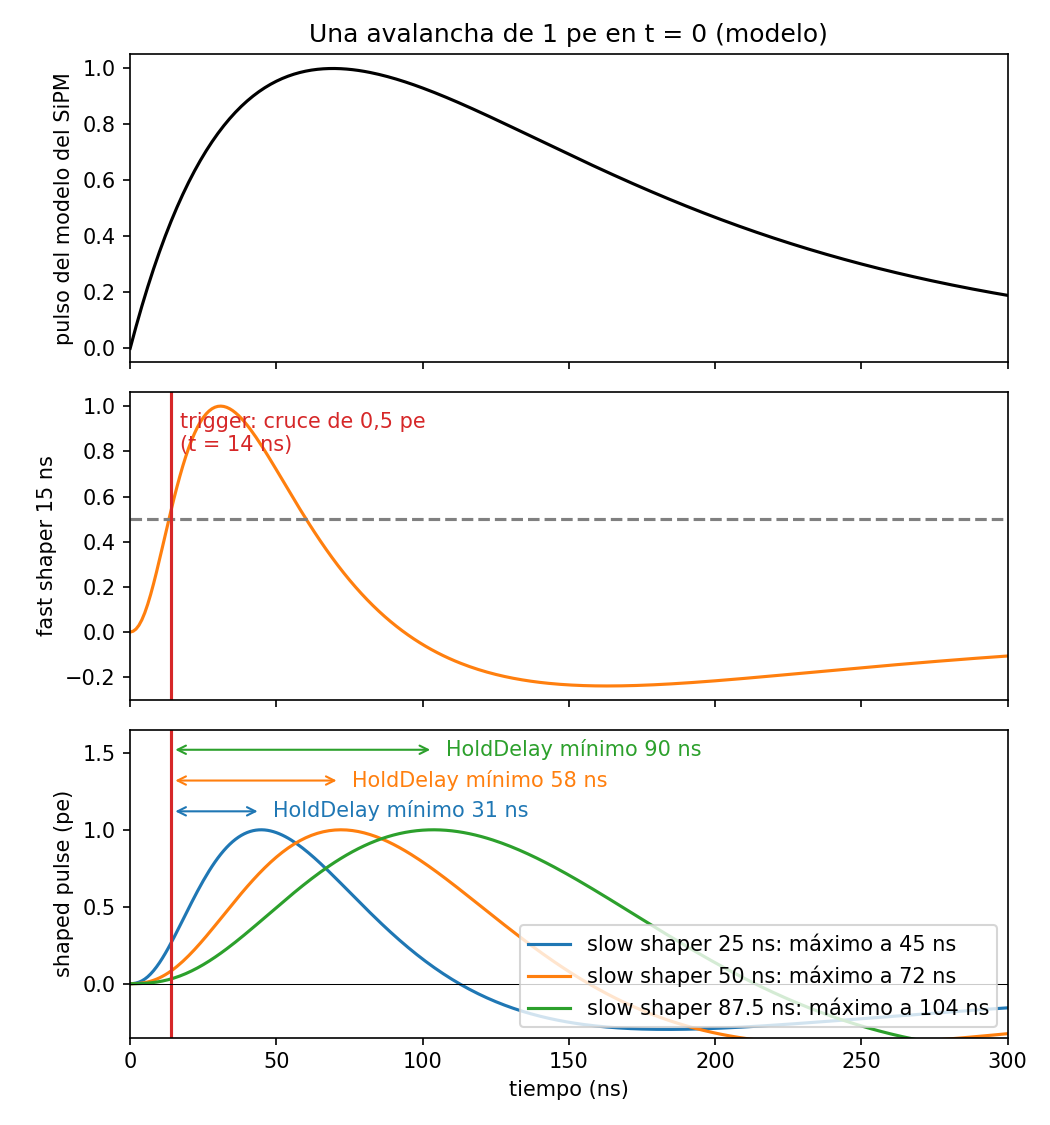
\includegraphics[width=0.55\textwidth]{mecanismo_ps.png}
\caption{Una avalancha de 1~fotoelectrón en $t = 0$, según el modelo de la
simulación. {\bf Arriba}, el pulso del SiPM, normalizado a 1 en su máximo.
{\bf En el centro}, la salida del fast shaper: el canal se dispara cuando
cruza 0,5~fotoelectrones, a 14~ns. {\bf Abajo}, la salida del slow shaper a
25, 50 y 87,5~ns; las flechas marcan el tiempo entre el trigger y el máximo
(31, 58 y 90~ns), el \texttt{HoldDelay} mínimo para que el peak stretch lo
recoja, sin contar la latencia de la tarjeta.}
\label{fig:mecanismo}
\end{figure}

\begin{itemize}
\item Cada avalancha del SiPM produce un pulso que sube hasta su máximo en
  69~ns y cae con una constante de 100~ns (Figura~\ref{fig:mecanismo},
  arriba). La subida la marca la recarga de la celda, unos 50~ns, y la
  caída el producto de la capacitancia del SiPM por la resistencia de
  entrada, 2000~pF $\times$ 50~$\Omega$. Su carga es la de un fotoelectrón
  (pe).
\item El pulso entra en dos preamplificadores en paralelo: el de alta
  ganancia (HG), para señales de pocos pe, y el de baja ganancia (LG), para
  los cientos de pe que recibe un canal en un evento de 511~keV. Sus
  ganancias se fijan con \texttt{HG\_Gain} y \texttt{LG\_Gain}.
\item Cada preamplificador alimenta su slow shaper (SS), un filtro que
  convierte el pulso en una forma con un máximo bien definido
  (Figura~\ref{fig:mecanismo}, abajo). Su shaping time se fija con
  \texttt{HG\_ShapingTime} y \texttt{LG\_ShapingTime}, entre 12,5 y
  87,5~ns. Un shaping largo recoge más luz de un pulso largo, como los de
  BGO y CsI, y tiene menos ruido; uno corto separa mejor dos pulsos
  próximos.
\item En paralelo, el fast shaper (FS, 15~ns) y un discriminador disparan el
  canal cuando la señal cruza un umbral (Figura~\ref{fig:mecanismo},
  centro). En la A5202 el trigger del evento es el OR de los 64 canales, o
  un trigger periódico (PTRG), como en esta nota; el hold es común a los 64
  canales.
\item Desde el trigger, el chip sigue la salida de cada slow shaper y va
  guardando el valor más alto que alcanza; al llegar el hold deja de
  seguirla y conserva ese máximo (peak stretch). El hold tiene que llegar
  después del máximo del pulso, no necesariamente en él. La FPGA de la tarjeta manda el hold
  \texttt{HoldDelay} después del trigger, en pasos de 8~ns, más un retraso
  propio de la tarjeta (la latencia), que no conocemos. Después se
  digitalizan las dos ganancias de los 64 canales.
\end{itemize}

\subsection*{Pedestal y ruido}

\begin{itemize}
\item Sin señal, el valor que el chip guarda de la salida del slow shaper es un nivel fijo, el pedestal, distinto en
  cada canal, más una fluctuación, el ruido. El pedestal se resta; el ruido
  se suma a cada medida y entra en la resolución en energía y en la anchura
  de los picos de los espectros de un fotoelectrón (single photoelectron,
  SPE) con los que se calibra la ganancia.
\item El ruido de un preamplificador crece con la capacitancia de su
  entrada, y la de nuestros SiPM es grande, unos 2000~pF por canal: hay que
  medirlo con los SiPM conectados. Disminuye al alargar el shaping.
\item Por debajo de la tensión de ruptura (breakdown voltage, BV) el SiPM
  conserva su capacitancia pero no produce avalanchas, y el pedestal
  contiene solo el ruido electrónico. Por encima del BV aparecen los pulsos
  oscuros (dark pulses, DP), varios MHz en cada canal. El
  BV es 38,0~V a 25~$^\circ$C y baja 34~mV por grado; a temperatura
  ambiente, \texttt{HV\_Vbias} $\approx$ 36,5~V deja todos los canales entre
  1 y 2~V por debajo.
\end{itemize}

\subsection*{Peak stretch y la ventana}

\begin{figure}[htbp!]
\centering
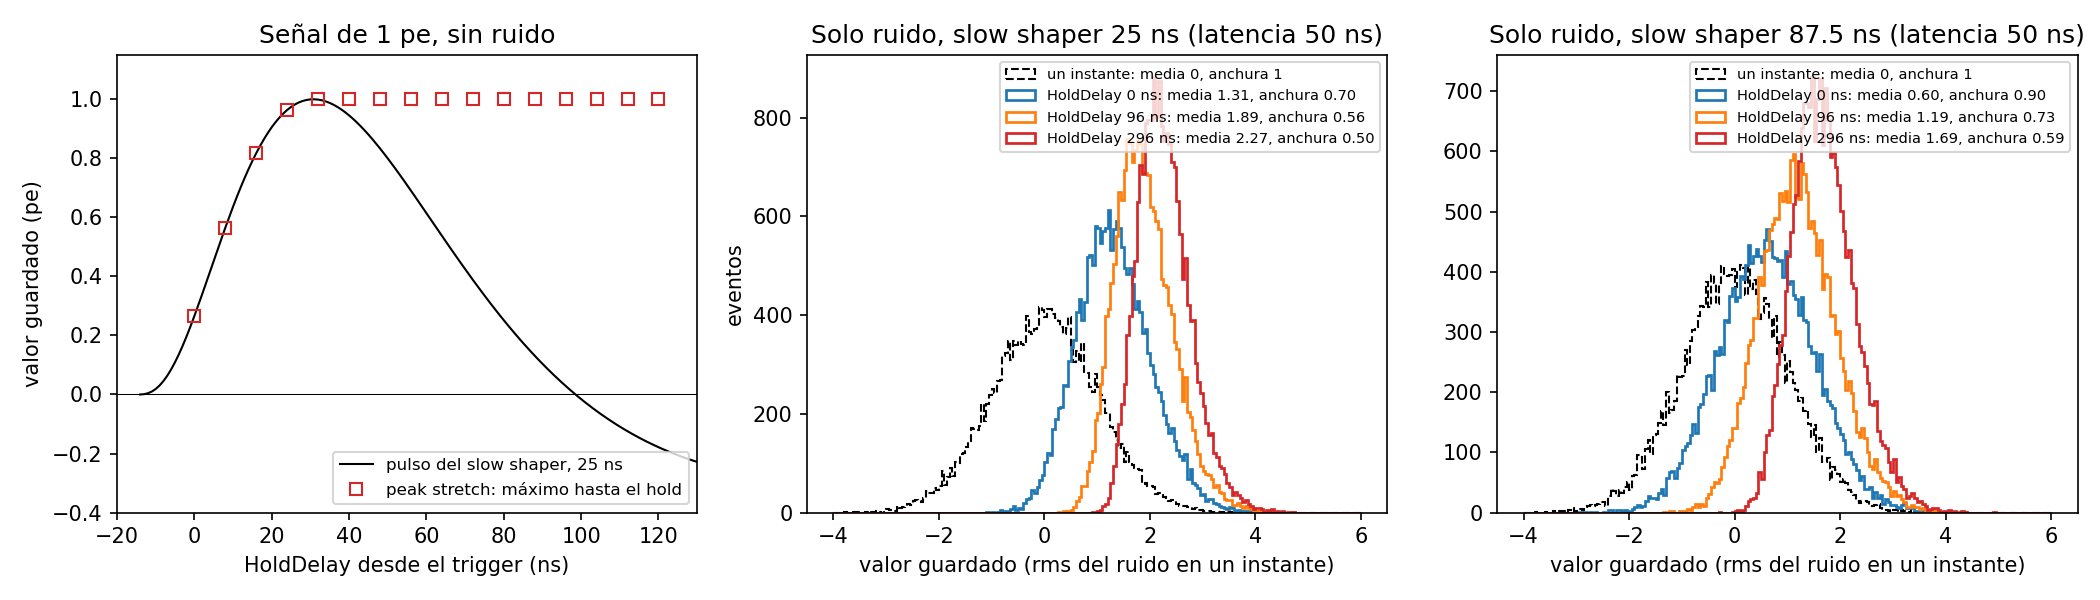
\includegraphics[width=\textwidth]{ventana.png}
\caption{Peak stretch, según un modelo sencillo con el pulso de la
Figura~\ref{fig:mecanismo}. {\bf Izquierda}, el valor guardado para una
avalancha de 1~pe con slow shaper de 25~ns, frente al \texttt{HoldDelay}:
crece hasta el máximo del pulso y se queda en él. {\bf Centro y derecha},
solo ruido (SiPM por debajo del BV), con slow shaper de 25 y 87,5~ns: el
valor guardado, en unidades del ruido en un instante, para tres
\texttt{HoldDelay} y una latencia supuesta de 50~ns. El pedestal sube y se
estrecha al alargar la ventana, más deprisa a 25~ns.}
\label{fig:ventana}
\end{figure}

\begin{itemize}
\item Con señal, el valor que el chip guarda de la salida del slow shaper
  (el máximo hasta el hold) crece con el \texttt{HoldDelay} hasta
  que la ventana contiene el máximo del pulso, y después se queda en una
  meseta (Figura~\ref{fig:ventana}, izquierda).
\item Con solo ruido, el chip guarda el máximo del ruido en la ventana. La
  ventana dura la latencia más el \texttt{HoldDelay}, así que con
  \texttt{HoldDelay} = 0~ns no es nula. Al alargarla, el máximo es cada vez
  mayor y varía menos de un evento a otro: el pedestal sube y se estrecha
  (Figura~\ref{fig:ventana}, centro y derecha).
\item El efecto depende del shaping. El ruido de un shaper corto cambia más
  deprisa, caben más fluctuaciones independientes en la misma ventana, y el
  pedestal se desplaza más: con 296~ns de \texttt{HoldDelay}, unas 2,3 veces
  el ruido en un instante a 25~ns y 1,7 veces a 87,5~ns.
\item Por eso la anchura medida no es directamente el ruido: es la del
  máximo del ruido en la ventana, y se compara con la que da el modelo para
  la misma ventana.
\end{itemize}

\subsection*{Para qué sirve cada ganancia}

\begin{itemize}
\item La baja ganancia mide la energía, con el shaping más largo, 87,5~ns,
  para no perder luz de BGO y CsI: por eso \texttt{LG\_ShapingTime} =
  87,5~ns en todos los runs.
\item La alta ganancia sirve para calibrar con los DP (menú~3): los picos de
  1, 2 y 3~pe dan la ganancia de cada canal, que se pasa a la baja ganancia
  con el cociente entre las dos ganancias.
\item Para calibrar, un shaping largo es malo: con varios MHz de DP por
  canal, a 87,5~ns los pulsos se apilan y los picos de SPE se borran; con un
  shaping corto se separan. Pero un shaping corto tiene más ruido, y ese
  ruido es la anchura de cada pico. El paso~1 mide el ruido en los tres
  shapings candidatos para calibrar, 25, 50 y 87,5~ns; el menú~3 mide los
  espectros de SPE en los mismos, y con los dos se elige el mejor. El run a
  87,5~ns da además el ruido de la baja ganancia al shaping de energía, el
  que entra en la resolución.
\end{itemize}

\section*{Programa de festejos}

\noindent {\bf Setup}
\begin{itemize}
\item {\bf Acción:}
  \begin{itemize}
  \item Montar sin cristal, con los SiPM conectados.
  \item Partir de la configuración de producción y cambiar en la pestaña
    {\bf Acquisition} solo los parámetros de la Sección~\ref{sec:janus}.
  \item \texttt{HV\_Vbias} de forma que los SiPM queden entre 1 y 2~V por
    debajo del BV (Sección~\ref{sec:medida}): unos 36,5~V, en lugar de los 45,4~V de
    producción. Fijarlo antes de lanzar el run, no durante.
  \item Guardar la configuración con {\bf Save config}.
  \item En la pestaña {\bf Hardware}, encender el HV de la tarjeta y esperar
    a que Vmon e Imon estén estables.
  \end{itemize}
\item {\bf Resultado:} cada run se para solo a los 10\,000 eventos. El DAQ
  le asigna un número \texttt{N} y escribe \texttt{run\_N.0000.h5} (para cada
  evento y canal, la alta y la baja ganancia, junto con la configuración del
  run, la temperatura y la tensión) y \texttt{run\_N.histograms.h5} (los
  histogramas de cada canal).
\item {\bf Precaución:} el run dura 10~s y termina antes de que dé tiempo a
  mirarlo en vivo. Al acabar el primero, mirar en la pestaña {\bf Plots}
  los histogramas guardados del espectro de alta ganancia de algunos
  canales: debe ser una sola gaussiana,
  sin pico de 1~pe a su derecha. Si aparece, los SiPM dan
  avalanchas: bajar \texttt{HV\_Vbias} 0,5~V y repetir.
\end{itemize}

\noindent {\bf Paso 1: ruido frente al shaping de la alta ganancia}
\begin{itemize}
\item {\bf Acción:}
  \begin{itemize}
  \item \texttt{HoldDelay} = 0~ns.
  \item \texttt{LG\_ShapingTime} = 87,5~ns.
  \item Un run con \texttt{HG\_ShapingTime} = 25~ns.
  \item Un run con \texttt{HG\_ShapingTime} = 50~ns.
  \item Un run con \texttt{HG\_ShapingTime} = 87,5~ns.
  \end{itemize}
\item {\bf Resultado:} 3 runs, cada uno con sus dos ficheros. Cada cambio
  de shaping es un run nuevo con su número: anotarlo en el logbook junto al
  shaping.
\item {\bf Análisis:} el de la Sección~\ref{sec:datos}: para cada run y
  canal, la media (pedestal) y la anchura (ruido) de la alta y la baja
  ganancia.
\end{itemize}

\noindent {\bf Paso 2: pedestal frente al HoldDelay}
\begin{itemize}
\item {\bf Acción:}
  \begin{itemize}
  \item \texttt{HG\_ShapingTime} = 25~ns.
  \item Un run con \texttt{HoldDelay} = 96~ns.
  \item Un run con \texttt{HoldDelay} = 200~ns.
  \item Un run con \texttt{HoldDelay} = 296~ns (lo que la tarjeta aplica con
    los 300~ns de producción).
  \item Un run con \texttt{HoldDelay} = 400~ns.
  \item Un run con \texttt{HoldDelay} = 496~ns.
  \item El de 0~ns ya está hecho en el paso 1.
  \end{itemize}
\item {\bf Resultado:} 5 runs, cada uno con sus dos ficheros.
\item {\bf Análisis:} el mismo que en el paso 1. Al alargar la ventana, el
  chip guarda el máximo del ruido en un intervalo más largo, y el pedestal
  sube y se estrecha. La baja ganancia, a 87,5~ns en todos los runs, da en
  los mismos runs su pedestal frente a la ventana al shaping de las medidas
  de energía, que se leen en baja ganancia. Esta es la parte electrónica del
  pedestal que verán esas medidas; la parte de los DP se mide en los menús 2
  y 3.
\end{itemize}

\noindent {\bf Paso 3: estabilidad}
\begin{itemize}
\item {\bf Acción:} repetir el primer run del paso 1
  (\texttt{HG\_ShapingTime} = 25~ns, \texttt{HoldDelay} = 0~ns).
\item {\bf Resultado:} 1 run con sus dos ficheros.
\item {\bf Análisis:} el pedestal debe coincidir con el del primer run; si
  se ha movido, la temperatura o la tensión han cambiado durante la sesión.
\end{itemize}

\section*{Qué necesita el cocinero}

\begin{itemize}
\item De cada run, los dos ficheros \texttt{.h5}.
%que se descargan en la
 % pestaña {\bf Runs}: seleccionar el run y pulsar {\bf Download} en cada
 % fichero de la lista {\bf Artifacts}.
\item Una fila por run en el logbook de la hoja de Google (nota 0). La
  configuración, la temperatura y la tensión están también dentro de los
  ficheros.
\item Si algo no se comporta como espera el menú, para y grita.
\end{itemize}

\section{Cómo entra la medida en el modelo}
\label{sec:razon}

\begin{itemize}
\item El ruido electrónico entra en la resolución en energía y en la
  anchura de los picos de SPE. La simulación lo estima, pero la estimación
  puede quedarse corta: necesitamos datos.
\item El modelo de la simulación supone 0,1~pe de ruido en alta ganancia con
  shaping de 87,5~ns y 3~V de overvoltage (tensión por encima del BV). El
  ruido es fijo en carga, y la carga de un pe es proporcional al
  overvoltage, así que a 5~V son 0,06~pe. Supone además que el ruido crece
  como $(87{,}5~\mathrm{ns}/t_p)^{1/2}$ al acortar el peaking time $t_p$, y
  que la baja ganancia tiene el mismo ruido en cuentas de ADC que la alta.
  Estas medidas nos permiten entender lo realistas que son estas
  suposiciones.
\item El modelo calcula el máximo del ruido en la ventana de cada run, la
  latencia más el \texttt{HoldDelay}. La latencia, que no conocemos, se
  ajusta con los runs del paso~2.
\end{itemize}

\section{Parámetros del DAQ (A5202)}
\label{sec:janus}

\begin{center}
\small
\begin{tabular}{p{0.3\textwidth} p{0.6\textwidth}}
\hline
parámetro & valor \\
\hline
\texttt{HV\_Vbias} & el que deje la tensión en cada SiPM entre 1 y 2~V por
debajo del BV: unos 36,5~V a temperatura ambiente \\
\texttt{HV\_IndivAdj} & 0 (como en producción), el mismo en los tres
estudios \\
\texttt{AcquisitionMode} & SPECTROSCOPY \\
\texttt{BunchTrgSource} & PTRG (trigger periódico, independiente de la señal) \\
\texttt{PtrgPeriod} & 1~ms: 10\,000 eventos en 10~s \\
\texttt{HG\_ShapingTime} & 25, 50 o 87,5~ns, según el run \\
\texttt{LG\_ShapingTime} & 87,5~ns \\
\texttt{HoldDelay} & 0~ns (pasos 1 y 3); 96, 200, 296, 400 o 496~ns
(paso 2): múltiplos de 8~ns, el paso de la tarjeta \\
\texttt{HG\_Gain}, \texttt{LG\_Gain} & 55 (como en producción), los mismos
en los tres estudios \\
\texttt{GainSelect} & BOTH \\
\texttt{ZS\_Threshold\_HG}, \texttt{ZS\_Threshold\_LG} & 0 (sin zero
suppression: hay que leer todos los canales en todos los eventos), también
en los umbrales por canal si la configuración los tiene \\
\texttt{EnableServiceEvents} & activado (guarda la temperatura y la tensión
medidas) \\
\texttt{ChEnableMask0}, \texttt{ChEnableMask1} & todos los canales
({\bf Configure channels}, {\bf Enable all}) \\
\texttt{StopRunMode}, \texttt{PresetCounts} & PRESET\_COUNTS, 10000 \\
{\bf Store run histograms} & activado (al final de la categoría RunCtrl) \\
\hline
\end{tabular}
\end{center}

\section{Análisis}
\label{sec:datos}

\begin{itemize}
\item \sloppy Cada run que lanzas genera \texttt{run\_N.0000.h5}; los datos están en la tabla
  \path{/events/spectroscopy/observations}: una fila por evento y canal,
  con las columnas \texttt{channel}, \texttt{high\_gain} y
  \texttt{low\_gain}.
\item Para cada canal y cada ganancia, una gaussiana ajustada al espectro.
  Su media es el pedestal y su sigma la anchura, los dos en cuentas de ADC.
  La anchura es la del máximo del ruido en la ventana, no directamente el
  ruido (Sección~\ref{sec:medida}).
  Para comparar runs se usa la mediana sobre los 64 canales. Un canal con
  una cola o un segundo pico tiene avalanchas o ruido de otro origen, y se
  anota aparte.
\item {\bf Paso a fotoelectrones:} el ruido en pe es el ruido en cuentas de
  ADC dividido por la ganancia en cuentas de ADC por pe, que miden los runs
  de calibración con SPE. Hay que usar la ganancia medida con el mismo
  shaping y el mismo \texttt{HG\_Gain}.
\end{itemize}

\section{Lo que se espera, según el modelo}

\begin{itemize}
\item {\bf Ruido de la alta ganancia, en pe de 5~V} (los de la calibración),
  en un instante: 0,06 a 87,5~ns, 0,08 a 50~ns y 0,11 a 25~ns. Las
  anchuras medidas con \texttt{HoldDelay} = 0~ns saldrán algo menores, sobre
  todo a 25~ns, porque la ventana no es nula.
\item {\bf Prueba sin ganancia:} el cociente entre el ruido a un shaping y
  el ruido a 87,5~ns, en cuentas de ADC, no depende de la ganancia. El
  modelo da 1,32 a 50~ns y 1,87 a 25~ns en un instante; con una latencia de
  unos 50~ns, los cocientes medidos serán más bien 1,2 a 1,3 y 1,5 a 1,7.
\item {\bf Baja ganancia:} el mismo ruido en cuentas de ADC que la alta a
  87,5~ns (run de 87,5~ns del paso 1, donde las dos tienen el mismo
  shaping).
\item {\bf Pedestal:} distinto en cada canal, estable entre runs. En el paso
  2, más alto y más estrecho cuanto más largo es el \texttt{HoldDelay}.
\end{itemize}

\end{document}
